% KrF_IB overview: how accurate LIGHT v0_5 (Kr/F2) and LIGHT_Kr
% (v0_5, pure Kr) are, their energy ladders, and every reaction rate.
%
% Where the numbers come from:
%   - Accuracy, uncertainty and reference-point numbers: the models' own
%     generated overviews, code/LIGHT/docs/accuracy_overview_v0_5.pdf
%     and code/Kr_LIGHT/docs/accuracy_overview_v0_5.pdf (code md5
%     eac04189da72, its run cache current on 2026-10-20).
%   - The energy ladders: the figures of those two overviews, embedded.
%   - Appendices A and B (rates, bands, species energies): generated from
%     the code by make_overview.py.
% Build (from KrF_IB/overview):
%   /usr/bin/python3 make_overview.py
%   latexmk -pdf overview.tex && cp build/overview.pdf ../overview.pdf
\documentclass[11pt]{article}
\usepackage[a4paper,margin=2.2cm]{geometry}
\usepackage[utf8]{inputenc}
\usepackage[T1]{fontenc}
\usepackage[scaled=0.95]{helvet}
\renewcommand{\familydefault}{\sfdefault}
\usepackage{amsmath}
\usepackage{sansmath}
\sansmath
\usepackage{booktabs,tabularx,array,longtable}
\usepackage{pdflscape}
\usepackage{xcolor}
\usepackage{float}
\usepackage{enumitem}
\usepackage{graphicx}
\usepackage[hidelinks]{hyperref}
\setlist{nosep, leftmargin=1.2em}
\setlength{\parindent}{0pt}
\setlength{\parskip}{5pt}
\definecolor{ink2}{HTML}{52514E}
\definecolor{accent}{HTML}{1F5A96}
\renewcommand{\topfraction}{0.95}
\renewcommand{\textfraction}{0.03}

\newcommand{\unit}[1]{\ensuremath{\,\mathrm{#1}}}
\newcommand{\el}{\ensuremath{\mathrm{e}^-}}
\newcommand{\Krs}{Kr\ensuremath{^*}}
\newcommand{\Krpp}{Kr\ensuremath{^{**}}}
\newcommand{\Krp}{Kr\ensuremath{^+}}
\newcommand{\Krtp}{Kr\ensuremath{_2^+}}
\newcommand{\Krts}{Kr\ensuremath{_2^*}}
\newcommand{\KrtF}{Kr\ensuremath{_2}F\ensuremath{^*}}
\newcommand{\Ft}{F\ensuremath{_2}}
\newcommand{\Edep}{\ensuremath{E_\mathrm{dep}}}
\newcommand{\x}{\ensuremath{\times}}
\definecolor{hlbg}{HTML}{FFE97A}
% the two models' headline uncertainties, highlighted and bold
\newcommand{\unc}[1]{\colorbox{hlbg}{\textbf{#1}}}

% generated by make_overview.py: do not edit
\newcommand\nrowsLight{59}
\newcommand\nzeroLight{11}
\newcommand\noptLight{2}
\newcommand\nbandsLight{17}
\newcommand\nspeciesLight{12}
\newcommand\nrowsKr{219}
\newcommand\nzeroKr{31}
\newcommand\noptKr{0}
\newcommand\nbandsKr{22}
\newcommand\nspeciesKr{10}

\makeatletter
% \input inside a tabular leaves end-of-file tokens before \bottomrule
\newcommand\tabinput[1]{\@@input generated/#1.tex }
\makeatother
\setlength{\emergencystretch}{2em}

\begin{document}

{\LARGE\bfseries KrF\_IB models: accuracy, energy ladders and reaction rates}\par
\vspace{4pt}
{\color{ink2} LIGHT v0\_5 (Kr/\Ft, the KrF laser gas) and LIGHT\_Kr v0\_5 (pure
krypton), in \texttt{code/LIGHT/v0\_5/} and \texttt{code/Kr\_LIGHT/v0\_5/},
20 October 2026}
\vspace{6pt}

\textbf{Bottom line.}
\begin{itemize}
\item \textbf{LIGHT v0\_5} (\nrowsLight{} rows on \nspeciesLight{} species). It
  reproduces the KrF(B,C) decays its rate fit used within 6.1\,\% rms, and
  the decays no fit used within 11.7\,\% rms. At the Tahoma laser it gives the
  small-signal gain to $-6$\,\%, the absorption to $-25$\,\%, the net gain to
  $-2$\,\%, the saturation intensity to $+4$\,\% and the formation efficiency
  to $-3$\,\%. \textbf{The propagated uncertainty of its own inputs is
  \unc{$\pm$\,40\,\%}}: $\pm 40$\,\% on Tahoma's net gain, $\pm 38$\,\% on the
  248-nm share (5.68\,\% of \Edep{}, $\pm 2.17$ points), $\pm 33$ and
  $\pm 37$\,\% on Tahoma's gain and absorption. Its largest errors:
  \begin{itemize}
  \item Hakuta et al.'s C--A decays, 19.3 and 34.1\,\% rms;
  \item Burnham and Searles' KrF(B) lifetime, $-22.3$\,\%;
  \item Kleikamp et al.'s Kr pressure optimum, $-37$\,\%, and their \Ft{}
    optimum not reproduced at all.
  \end{itemize}
\item \textbf{LIGHT\_Kr v0\_5} (\nrowsKr{} rows on \nspeciesKr{} species). The
  parts that measurements reach are close:
  \begin{itemize}
  \item drift velocity within 2.8\,\% rms;
  \item ionization coefficient within 9.9\,\% rms at 50--300\,Td;
  \item electroluminescence yield at 0.99--1.04 of the measurement;
  \item e-beam VUV efficiency $+29$\,\% (low pump) and $-3$\,\% (high pump).
  \end{itemize}
  Its headline output is not close. The 147-nm share at the reference point
  is 6.08\,\% of \Edep{} with \textbf{a propagated uncertainty of
  \unc{$\pm$\,115\,\%}} ($\pm 7.0$ points). That term is dominated by electron collisions with
  \Krts{}, which nothing measures, and no measurement tests the field-driven
  regime the model is built for.
\end{itemize}
Both models are 0-D and predictive only: no rate is tuned to a device
measurement. Device and beam data only score the model; LIGHT's KrF(B,C)
constants are a joint fit to decay data, and LIGHT\_Kr's cross sections are
trained on swarm data alone. The energy ladders are in Sections~\ref{sec:light-ladder}
and~\ref{sec:kr-ladder}, and every reaction rate is in Appendices~\ref{app:light}
and~\ref{app:kr}.

\begin{table}[H]
\small
\begin{tabularx}{\textwidth}{@{}lXX@{}}
\toprule
 & LIGHT v0\_5 & LIGHT\_Kr v0\_5 \\
\midrule
gas & Kr/\Ft{} (0.5\,\% \Ft{} at the reference point) & pure Kr \\
code & \texttt{code/LIGHT/v0\_5/} (\texttt{run\_v0\_5.py}) & \texttt{code/Kr\_LIGHT/v0\_5/} (\texttt{run\_v0\_5.py}) \\
network & \nrowsLight{} rows, \nspeciesLight{} species, \nbandsLight{} bands (\nzeroLight{} rows at 0 by default) & \nrowsKr{} rows, \nspeciesKr{} species, \nbandsKr{} bands (\nzeroKr{} rows at 0 by default) \\
electrons & kinetic EEDF (two-term Boltzmann with e--e collisions) by default; two-temperature closure as the fast option & the same \\
reference point & 1\,atm, 300\,kW\,cm$^{-3}$ for 1\,\textmu s, run to 2\,\textmu s & the same, pure Kr \\
headline output & 248\,nm: 5.73\,\% of \Edep{} (kinetic), 5.7\,\% (two-temp.) & 147\,nm: 6.08\,\% of \Edep{} (kinetic), 5.58\,\% (two-temp.) \\
\textbf{its uncertainty} & \unc{$\pm$\,40\,\%} (quadrature, 22 inputs; $\pm 38$\,\% on the 248-nm share) & \unc{$\pm$\,115\,\%} (quadrature, 24 inputs and the cross sections' posterior) \\
what v0\_5 adds & K76 (\el{} + \Krs{} $\to$ \el{} + \Krpp{}) on Jung et al.'s measured cross sections; Kleikamp et al.'s laser held out & the electrons' collisions with excited Kr and \Krts{} (Vriens--Smeets), each 5s$\to$5p pair at its own threshold \\
accuracy source & \nolinkurl{LIGHT/docs/accuracy_overview_v0_5.pdf} & \nolinkurl{Kr_LIGHT/docs/accuracy_overview_v0_5.pdf} \\
\bottomrule
\end{tabularx}
\caption{The two models at a glance.}
\end{table}

% ======================================================================
\section{LIGHT v0\_5: the Kr/\Ft{} model}

\textbf{What it is.} LIGHT is a 0-D model of KrF laser gas. It is one uniform
box at constant volume, and a given power goes into its electrons. It
follows that energy into excitation, ionization, KrF(B,C) and \KrtF{}
formation, the 248, 272, 275 and 420-nm and 147-nm bands, heat and the
electron gas, and its energy ledger closes by construction.
v0\_5 is v0\_4 with K76 ($\el + \Krs \to \el + \Krpp$) on the cross
sections Jung et al.\ measured out of the metastable levels, in place of
a 1976 fit, and with a second laser, Kleikamp et al.'s, held out.
Everything here is from v0\_5's generated accuracy overview.

\subsection{Against the data}

\begin{table}[H]
\small
\begin{tabularx}{\textwidth}{@{}Xllll@{}}
\toprule
quantity & measured & LIGHT & error & role \\
\midrule
energy ledger closure & & $<3.4\times10^{-14}$ & & bookkeeping \\
KrF(B) decay vs Kr and \Ft{}, Eden 1978 & & & rms 2.3, 3.2\,\% & trains \\
KrF(B,C) slow decay, Gadomski 1992 Figs.\ 1, 2 & & & rms 6.1, 4.2\,\% & trains \\
C/B emission ratio at 300\,K, Yu \& Setser 1990 & $0.16\pm0.02$ & & $-0.5$\,\% & trains \\
KrF(B,C) decays, Xu 1993 Figs.\ 5--7 & three figures & & rms 11.7\,\% & held out \\
decay constants at 50, 100\,Torr Kr, Xu 1993 & $5.0, 6.2\times10^7$\,s$^{-1}$ & \x0.91, \x0.97 & $-9$, $-3$\,\% & structure check \\
C/B ratio 230\,K over 300\,K, Yu \& Setser & $1.30\pm0.06$ & & $-8.4$\,\% & held out \\
C--A decays, Hakuta 1990 & two figures & & rms 19.3, 34.1\,\% & held out, in conflict \\
$\tau_B$, Burnham \& Searles 1977 & $9.0\pm0.6$\,ns & & $-22.3$\,\% & held out, in conflict \\
\midrule
Tahoma small-signal gain $g_0$, kinetic EEDF & 6.39\,\%/cm & 5.99 & $-6$\,\% & device, score only \\
Tahoma absorption $\alpha_0$ & 1.11\,\%/cm & 0.83 & $-25$\,\% & device, score only \\
Tahoma net gain $g_0-\alpha_0$ & 5.28\,\%/cm & 5.16 & $-2$\,\% & device, score only \\
Tahoma saturation intensity (two-temp.) & $1.4\pm0.1$\,MW/cm$^2$ & 1.45 & $+4$\,\% & device, score only \\
Tahoma formation efficiency $g_0I_\mathrm{sat}/P_\mathrm{in}$ & 0.27 & 0.261 & $-3$\,\% & device, score only \\
Tahoma loss in pure Kr, 257.3\,nm & 0.67\,\%/cm & 0.24 & \x0.36 & rough check \\
VUV yield of pure Kr at low pump, Morozov 2008 & $0.42\pm0.05$ & 0.55 & $+32$\,\% & held out (v0\_3's run) \\
\midrule
Kr pressure optimum, Kleikamp 1986, \Ft{} 10\,mbar & 2\,atm & 1.26\,atm & $-37$\,\% & device, held out \\
\Ft{} pressure optimum, Kr 2\,atm & 10\,mbar & $>30$\,mbar & not reproduced & device, held out \\
three-body KrF$^*$ + Kr quenching their balance deduces & $4.6\times10^{-31}$\,cm$^6$/s & $1.02\times10^{-30}$ & \x2.2 & device, score only \\
\bottomrule
\end{tabularx}
\caption{LIGHT v0\_5 against the data, every band at its default.
An error is model less measurement over the measurement, signed for one
value and rms over a set. ``Trains'': the KrF(B,C) constants are a joint
fit to these decays; every device row only scores the model. Tahoma's
saturation intensity and formation efficiency and the Kleikamp optimum run
on the two-temperature closure; the kinetic EEDF moves Tahoma's numbers by
about 1\,\%.}
\end{table}

\subsection{Propagated uncertainty: \unc{$\pm$\,40\,\%}}

Each of 22 inputs is set alone to the two ends its source allows: 17 bands,
3 measured constants with quoted errors and 2 cross sections. Half the
difference between the two runs is that input's term, and the terms add in
quadrature. That sum is indicative, not a confidence interval, and the
summed excursions are the ceiling of the spread.

\begin{table}[H]
\small
\begin{tabularx}{\textwidth}{@{}lllX@{}}
\toprule
output & value & quadrature & largest terms \\
\midrule
248-nm share & 5.68\,\% of \Edep{} & $\pm 2.17$ pts ($\pm 38$\,\%) & the trimer's $(T_g/300)^n$ ($\pm 1.70$), \Krts{} + F $\to$ KrF(B) ($\pm 0.91$), KrF(B,C) + F ($\pm 0.88$), \el{} + \Krs{} ionization ($\pm 0.29$); excursions $-6.85$/$+2.46$ pts \\
Tahoma $g_0$ & 5.93\,\%/cm & $\pm 33$\,\% & trimer law ($\pm 1.55$), KrF$^*$ per ion-ion recombination ($\pm 0.75$), $\sigma_\mathrm{se}$ ($\pm 0.71$), KrF(B,C) + F ($\pm 0.47$); measurement 0.2 units away \\
Tahoma $\alpha_0$ & 0.82\,\%/cm & $\pm 37$\,\% & \KrtF{} + \Ft{} ($\pm 0.18$), \KrtF{} + F ($\pm 0.16$), $\sigma(\KrtF)$ ($\pm 0.12$), trimer law ($\pm 0.10$); measurement 0.9 units away \\
Tahoma $g_0-\alpha_0$ & 5.11\,\%/cm & \unc{$\pm$\,40\,\%} & measurement 0.1 units away \\
\bottomrule
\end{tabularx}
\caption{LIGHT's propagated uncertainty (two-temperature closure). Every
Tahoma measurement lies within one quadrature unit. Not propagated: the
electron-impact cross sections (the band \textsf{k\_5s5p} carries the
5s$\to$5p set's $\pm 35$--40\,\%) and the fitted KrF(B,C) set, which the
training decays pin at 6.1\,\% rms.}
\end{table}

\subsection{The reference point}

At 1\,atm, 0.5\,\% \Ft{}, 300\,kW\,cm$^{-3}$ for 1\,\textmu s, run to 2\,\textmu s:

\begin{table}[H]
\small\centering
\begin{tabular}{@{}lrr@{}}
\toprule
percent of \Edep{} unless stated & kinetic EEDF & two-temperature \\
\midrule
248\,nm, KrF B--X & 5.73 & 5.7 \\
272\,nm, KrF B--A / 275\,nm, C--A & 0.183 / 0.829 & 0.2 / 0.8 \\
420\,nm, \KrtF{} & 4.21 & 3.9 \\
147\,nm, \Krts{} & 4.8 & 4.6 \\
near IR, 5p$\to$5s & 0.28 & 0.3 \\
heat, reactions / elastic & 72.6 / 1.8 & 71.6 / 3.4 \\
KrF(B) formed & 24.2 & 23.0 \\
$g_0$ / $\alpha$, 500--1000\,ns (\%/cm) & 3.79 / 0.67 & 3.96 / 0.64 \\
$T_g$ at the end (K) & 738 & 742 \\
$T_e$, pulse mean (eV) & 2.96 & 5.68 \\
\bottomrule
\end{tabular}
\caption{LIGHT's reference point. What moves it is the 5s$\leftrightarrow$5p
cycle: the electrons pump 79--81\,\% of the \Krs{} formed up to the 5p rung,
which relaxes on Kr, and each cycle's 1.385\,eV heats the gas (33.7\,\% of
the input). Numerically, the ledger closes below $10^{-14}$ and the
kinetic and model energy balances agree to $6.6\times10^{-6}$.}
\end{table}

\subsection{The energy ladder}\label{sec:light-ladder}

\begin{figure}[H]
\centering
\includegraphics[page=9, trim=40 205 35 40, clip, width=\textwidth]{../code/LIGHT/docs/accuracy_overview_v0_5.pdf}
\caption{LIGHT v0\_5's energy ladder, in eV
above ground-state Kr and \Ft{} at rest. A bar is a species at its
formation energy and a dashed bar a pair; an arrow is a row, labelled with
its id (Appendix~\ref{app:light}). Solid: default network; dotted: a band
whose default is 0 (Q2FF, K26C, K26X, K108C, K108X, K2F\_F, PEN\_KR2,
KSTEP\_S, KSTEP\_P, QF, QFC); dashed: the optional group \texttt{electron}.
A photon's arrow drops by its quantum and the red squiggle is the heat its
lower state gives the gas; a red stub is a quench. KrF(B) lies 5.54\,eV
below Kr$^+$ + F$^-$ and 5.06\,eV above Kr + F, and the 248-nm photon carries
5.00\,eV of that. The 5p rung lies 1.39\,eV above \Krs{}. G6 and VIB1--4 move
nothing between levels and are not drawn. From
\texttt{LIGHT/docs/accuracy\_overview\_v0\_5.pdf}, Figure~1.}
\end{figure}

\begin{table}[H]
\small\centering
\begin{tabular}{@{}lr@{}}
\toprule
species & $E_\mathrm{form}$ (eV) \\
\midrule
\tabinput{species_light}
\bottomrule
\end{tabular}
\caption{The rungs of LIGHT's ladder as the code books them
(\texttt{species.e\_form}): formation energy above ground-state Kr and
\Ft{}, which every row's energy release is the difference of.}
\end{table}

\subsection{Where LIGHT is not yet reliable}
\begin{itemize}
\item The trimer's rate at laser gas temperatures. Its temperature law,
  a calculation measured only to 425\,K, is the largest term of the
  propagated uncertainty. Kleikamp et al.'s laser finds LIGHT's quenching
  \x2.2 too strong at 362\,K, through a model-dependent constant.
\item The \Ft{}-side absorbers and KrF$^*$ + \Ft{}. The laser's \Ft{}
  optimum is not reproduced.
\item The rows with no measurement. \Krts{} + F, KrF(B,C) + F, \KrtF{} + F,
  \Krts{} + \Krts{} and the stepwise ionizations are bands at 0.
\item Two J\,=\,1 5s levels have no measured 5s$\to$5p cross section and use
  proxies; Jung et al.'s absolute scale is $\pm 35$--40\,\%.
\item The steady EEDF after the pulse, Hakuta's and Burnham \& Searles'
  conflicts, the absorbers as a diagnostic only, no cavity, and 0-D.
\end{itemize}

% ======================================================================
\section{LIGHT\_Kr v0\_5: the pure-krypton model}

\textbf{What it is.} LIGHT\_Kr is LIGHT with every fluorine species and row
removed, rebuilt for pure krypton. Its network has these parts:
\begin{itemize}
\item all 51 of Biagi's excitation levels at their own thresholds, with
  cross sections trained on swarm data;
\item the four 5s levels as separate species;
\item every measured 5s$\to$5p pair at its own threshold;
\item excimer formation out of each 5s level, and its redissociation by
  detailed balance;
\item Signorell's \Krtp{}.
\end{itemize}
v0\_5 adds the electrons' collisions with the excited atoms and with
\Krts{}. Where nothing is measured, the ionizations use Vriens and Smeets's
calculation, as bands from 0 to twice it. \Krts{}'s quenching and state
mixing by electrons are bands at 0. That cut the reference point's 147-nm
share from v0\_4's 31.22\,\% to 6.08\,\%.

\subsection{Against the data}

\begin{table}[H]
\small
\begin{tabularx}{\textwidth}{@{}Xlll@{}}
\toprule
test & measured & error & role \\
\midrule
energy ledger closure, reference point & & $4\times10^{-15}$ of \Edep{} & bookkeeping \\
energy balance at each of 30 nodes & & to $10^{-8}$ & bookkeeping \\
\midrule
drift velocity, 3 sets that agree, 79 pts & & rms 2.8\,\% & trains \\
ionization coefficient 50--300\,Td, 5 sets, 64 pts & & rms 9.9\,\% & trains \\
drift velocity, 8 sets that do not agree (1953--1992) & & rms 8 to 47\,\% by set & held out \\
characteristic energy $D_T/\mu$, Koizumi 1986, 26 pts & & rms 7.1\,\% (Biagi's file: 15.8\,\%) & validation \\
ionization coefficient $<$50\,Td, 5 sets, 36 pts & & mean $-36$\,\% (sets part by \x4.0) & held out by rule \\
electroluminescence yield 6--13.5\,Td, Mano 2022 & $0.113\,E/N-0.3$ & 0.99 to 1.04 of it & held out \\
superelastic return of 1s$_5$, 1s$_4$, 1s$_3$, Blagoev 1984 & 1.5, 5.2, $9.8\times10^{-10}$\,cm$^3$/s & \x5.3--6.6, \x5.5--9.5, \x0.5--1.2 & new, held out \\
Monte Carlo ionization coefficient, same cross sections, 20--50\,Td & & $+3.7$ to $-4.0$\,\% & solver check \\
\midrule
energy per ion pair $W$ under a beam, Saito 2003 & 23.9\,eV & $+10$\,\% & held out \\
excitations per ion pair, Saito 2003 & 0.55 & $+24$\,\% & held out \\
energy per excitation or ion, Saito 2003 & 15.4\,eV & $+1.0$\,\% & beam check \\
VUV efficiency, continuous e-beam, Morozov 2008 & $0.42\pm0.05$ & $+29$\,\% (2.5\,$\sigma$) & held out \\
VUV efficiency at $3\times10^5$\,W\,cm$^{-3}$, Eckstrom 1988 & near 0.46 & $-3$\,\% at 1\,atm & held out \\
\bottomrule
\end{tabularx}
\caption{LIGHT\_Kr v0\_5 against the data, every band at its default, on
the kinetic EEDF. Only swarm data train anything (seven factors on Biagi's
cross sections); every other row only scores the model. The swarm rows
compare the model as each experiment measures it (two-term solution \x{}
Monte Carlo ratios). No pure-krypton measurement in hand tests the
field-driven regime at the reference point's density.}
\end{table}

\subsection{Propagated uncertainty: \unc{$\pm$\,115\,\%}, and numerical accuracy}

Each of 24 inputs is set alone to its two ends, on both closures: 21 bands
and 3 measured constants. A calculated row's band runs from 0 to twice the
calculation. The trained cross sections add the spread of 12 (kinetic) and
40 (two-temperature) draws of their posterior.

\begin{table}[H]
\small
\begin{tabularx}{\textwidth}{@{}Xll@{}}
\toprule
input & its two ends & 147\,nm, kinetic (\% of \Edep) \\
\midrule
\el{} + \Krts{} $\to$ \Krtp{} + 2\el{}, scale on Vriens--Smeets & 0 to 2 & 15.43 to 4.47 \\
\el{} + \Krts{} $\to$ \el{} + \Krts(0$_u^+$), state mixing & 0 to $10^{-7}$\,cm$^3$/s & 6.08 to 12.44 \\
\el{} + \Krts{} $\to$ \el{} + 2Kr, quenching & 0 to $10^{-7}$\,cm$^3$/s & 6.08 to 1.27 \\
\Krs(1s$_4$) + 2Kr $\to$ \Krts{} + Kr & 1.3 to $9.2\times10^{-32}$\,cm$^6$/s & 4.29 to 6.08 \\
\el{} + \Krs{} $\to$ \Krpp{}, scale on Jung et al. & 0.6 to 1.4 & 7.06 to 5.46 \\
\el{} + \Krs{} $\to$ \Krp{} + 2\el{}, scale & 0 to 2 & 6.96 to 5.60 \\
\Krpp{} + Kr $\to$ \Krs{} + Kr & 3.0 to $17\times10^{-11}$\,cm$^3$/s & 7.11 to 6.08 \\
the trained cross sections & 12 posterior draws & $6.11\pm0.06$ \\
\midrule
\textbf{quadrature sum} (24 inputs) & & $\pm 7.0$ pts (\unc{$\pm$\,115\,\%}); two-temp.\ $\pm 7.2$ ($\pm 129$\,\%) \\
excursions summed by sign & & $-13.2$ / $+21.5$ pts \\
\bottomrule
\end{tabularx}
\caption{The largest terms of LIGHT\_Kr's propagated uncertainty on the
147-nm share (6.08\,\% kinetic, 5.58\,\% two-temperature). The first alone
makes 61\,\% of the quadrature sum's square. The full list of 24 is Table~2
of \texttt{Kr\_LIGHT/docs/accuracy\_overview\_v0\_5.pdf}.}
\end{table}

\textbf{Numerical error} is far below the physical uncertainty:
\begin{itemize}
\item The ledger closes to $4\times10^{-15}$ (kinetic) and $2\times10^{-14}$
  (two-temp.).
\item Halving the kinetic EEDF's renewal step moves the 147-nm share by
  $2\times10^{-6}$ of itself; doubling its energy cells moves it by
  $1\times10^{-3}$.
\item A tenfold tighter solver tolerance moves it by $8\times10^{-8}$.
\item Time-stepping the afterglow's EEDF instead of solving it steady moves
  it by $2\times10^{-4}$.
\item The two-temperature closure lies $-8$\,\% from the kinetic EEDF at
  the reference point and within 6\,\% at the scan's corners.
\end{itemize}

\subsection{The reference point}

\begin{table}[H]
\small\centering
\begin{tabular}{@{}lrr@{}}
\toprule
percent of \Edep{} unless stated & kinetic EEDF & two-temperature \\
\midrule
147\,nm, \Krts{} & 6.08 & 5.58 \\
near IR, 5p$\to$5s & 0.48 & 0.48 \\
heat, reactions and relaxation & 90.69 & 90.67 \\
heat, elastic collisions & 3.23 & 3.75 \\
\Krts{} formed that radiates / is ionized / redissociates (\%) & 28.5 / 56.9 / 14.0 & 26.0 / 59.9 / 13.5 \\
5s$\to$5p pumpings per \Krts{} formed, net & 25 & 24 \\
$T_e$, pulse mean (eV) & 1.57 & 1.53 \\
$n_e$, pulse mean (cm$^{-3}$) & $8.2\times10^{14}$ & $8.6\times10^{14}$ \\
$T_g$ at the end (K) & 856 & 859 \\
\bottomrule
\end{tabular}
\caption{LIGHT\_Kr's reference point at $t$\,=\,2\,\textmu s (1\,atm, 300\,K,
300\,kW\,cm$^{-3}$ for 1\,\textmu s). The 5s$\leftrightarrow$5p cycle turns
73.3\,\% of the input into heat, 102\,eV for each 147-nm photon. Over
pressure and power the share runs from 0 at 0.1\,atm to 19.85\,\% at 2\,atm
and 100\,kW\,cm$^{-3}$ (two-temperature closure).}
\end{table}

\subsection{The energy ladder}\label{sec:kr-ladder}

\begin{figure}[H]
\centering
\includegraphics[page=17, trim=12 532 40 36, clip, width=\textwidth]{../code/Kr_LIGHT/docs/accuracy_overview_v0_5.pdf}
\caption{LIGHT\_Kr v0\_5's energy ladder in eV above ground-state krypton at
rest; the four 5s levels are drawn side by side. Blue arrows are electron
impact, which takes its energy from the electron gas; K76r returns it.
KSTEP\_S and KSTEP\_P ionize the 5s levels (3.356--4.084\,eV) and the 5p rung
(2.696\,eV from 2p$_{10}$), EI ionizes \Krts{} (3.644\,eV), and SUPER (dotted)
returns a 5s level to the ground state. The dashed G2 is Penning ionization
of the 5s levels on one another. A red squiggle is heat: KPS relaxes the
5p rung on krypton, and PRAD radiates its gap in the near infrared. The
excimer forms out of each 5s level, redissociates by detailed balance
(AK8r), and radiates 8.43\,eV at 147\,nm onto the repulsive ground state.
C1's levels, 11.30--13.60\,eV, cascade to the 5p rung. MIX, the
Hornbeck--Molnar band and the resonance lines are not drawn. From
\texttt{Kr\_LIGHT/docs/accuracy\_overview\_v0\_5.pdf}, Figure~2.}
\end{figure}

\begin{table}[H]
\small\centering
\begin{tabular}{@{}lr@{}}
\toprule
species & $E_\mathrm{form}$ (eV) \\
\midrule
\tabinput{species_kr}
\bottomrule
\end{tabular}
\caption{The rungs of LIGHT\_Kr's ladder as the code books them
(\texttt{species.e\_form}), above ground-state krypton.}
\end{table}

\subsection{Where LIGHT\_Kr is not yet reliable}
\begin{itemize}
\item The electrons' collisions with \Krts{} decide the answer and are
  unmeasured. Its ionization is a calculation; its quenching and state
  mixing have neither measurement nor calculation (bands at 0, to Kannari's
  estimate).
\item The excimer's formation: the 1s$_5$ measurements spread \x2.5, 1s$_4$
  rests on one measurement, 1s$_3$ is a proxy, and the temperature law is
  measured at 200--400\,K while the reference point ends at 856\,K.
\item The superelastic returns are 5--9 times Blagoev et al.'s thermal
  rates for 1s$_5$ and 1s$_4$ (they move the reference point by $-0.5$\,\%).
\item The field-driven 5s$\leftrightarrow$5p cycle is unscored. The J\,=\,1
  levels use proxies, and the 5p rung's levels are assumed populated at the
  gas temperature.
\item The e-beam efficiency at low pump is $+29$\,\% off Morozov et al., and
  no process in the model explains it.
\item Not carried at all: Kr$_3^+$, Penning ionization between \Krs{} and
  \Krts{}, the other 5s transfers by electrons, and Kr$^+$ + 2\el{}.
\end{itemize}

% ======================================================================
\appendix
\newcommand{\ratehead}{%
  \toprule
  row & reaction & rate law & $k$, $T_e$\,=\,1\,eV & $k$, $T_e$\,=\,3\,eV & unit & bands & source (excerpt) \\
  \midrule}
\newcommand{\bandhead}{%
  \toprule
  band & rate & default & range & unit & rows that read it \\
  \midrule}

\begin{landscape}
\section{LIGHT v0\_5: every reaction rate}\label{app:light}

The \nrowsLight{} rows of the default network (\texttt{network.build()}, the
rows a default run integrates), in the code's order, with each row's rate
law and its rate constant evaluated by the model's own code
(\texttt{Model.\_k}) at $T_g$\,=\,300\,K, the 1-atm fill and every band at its
default. Electron rows are given for a Maxwellian at $T_e$\,=\,1 and 3\,eV;
a heavy-particle row's $k$ does not depend on $T_e$ (``same''). The model's
default closure is the kinetic EEDF solved during the run, so for electron
rows these Maxwellian values are a reference, not what a run uses. The
ion-ion rows include the Debye screening at $n_e$\,=\,$10^{14}$\,cm$^{-3}$.
\nzeroLight{} rows are 0 by default: they are bands with no measurement.
The source column is the start of each row's citation in
\texttt{v0\_5/network.py}; \texttt{v0\_5/SOURCES.md} says how each source
was read.

{\scriptsize
\setlength{\tabcolsep}{3pt}
\renewcommand{\arraystretch}{1.15}
\begin{longtable}{@{}>{\raggedright}p{1.6cm}>{\raggedright}p{3.4cm}>{\raggedright}p{5.0cm}p{1.6cm}p{1.6cm}p{0.95cm}>{\raggedright}p{1.6cm}>{\raggedright\arraybackslash}p{7.3cm}@{}}
\caption{LIGHT v0\_5's reaction rates.}\\
\ratehead
\endfirsthead
\ratehead
\endhead
\tabinput{rates_light}
\bottomrule
\end{longtable}
}

\textbf{Optional rows.} The group \texttt{electron} (\texttt{--add electron})
adds these \noptLight{} rows; a default run leaves them out.

{\scriptsize
\setlength{\tabcolsep}{3pt}
\begin{longtable}{@{}>{\raggedright}p{1.6cm}>{\raggedright}p{1.4cm}>{\raggedright}p{3.4cm}>{\raggedright}p{6.5cm}>{\raggedright\arraybackslash}p{10cm}@{}}
\toprule
row & group & reaction & rate law & source (excerpt) \\
\midrule
\tabinput{optional_light}
\bottomrule
\end{longtable}
}

{\scriptsize
\setlength{\tabcolsep}{3pt}
\begin{longtable}{@{}>{\raggedright}p{2.2cm}>{\raggedright}p{7.2cm}p{1.8cm}>{\raggedright}p{3.8cm}>{\raggedright}p{1.3cm}>{\raggedright\arraybackslash}p{6.6cm}@{}}
\caption{LIGHT v0\_5's bands (\texttt{network.BANDS}): rates carried with
a default and two ends. A rate with no measurement defaults to 0 and its
band runs to the largest published value. The propagated uncertainty runs
each band's two ends.}\\
\bandhead
\endfirsthead
\bandhead
\endhead
\tabinput{bands_light}
\bottomrule
\end{longtable}
}

\section{LIGHT\_Kr v0\_5: every reaction rate}\label{app:kr}

The \nrowsKr{} rows of the default network, in the code's order, evaluated
as in Appendix~\ref{app:light} ($T_g$\,=\,300\,K, 1\,atm, bands at their
defaults; electron rows on a Maxwellian at 1 and 3\,eV). \nzeroKr{} rows are 0
by default. A row marked $^\dagger$ leaves from one level of the 5p rung:
its $k$ is per atom in that level, and the model multiplies it by the
level's share of \Krpp{} at $T_g$ (98\,\% 2p$_{10}$ at 300\,K). The Kr
excitation rows run on Biagi's Magboltz 8.97 cross sections with v0\_3's
trained factors. The source column is the start of each row's citation in
\texttt{v0\_5/network.py}; \texttt{v0\_5/SOURCES.md} has the full sources.

{\scriptsize
\setlength{\tabcolsep}{3pt}
\renewcommand{\arraystretch}{1.15}
\begin{longtable}{@{}>{\raggedright}p{1.9cm}>{\raggedright}p{3.4cm}>{\raggedright}p{5.0cm}p{1.6cm}p{1.6cm}p{0.95cm}>{\raggedright}p{1.5cm}>{\raggedright\arraybackslash}p{7.1cm}@{}}
\caption{LIGHT\_Kr v0\_5's reaction rates.}\\
\ratehead
\endfirsthead
\ratehead
\endhead
\tabinput{rates_kr}
\bottomrule
\end{longtable}
}

{\scriptsize
\setlength{\tabcolsep}{3pt}
\begin{longtable}{@{}>{\raggedright}p{2.2cm}>{\raggedright}p{7.2cm}p{1.8cm}>{\raggedright}p{3.8cm}>{\raggedright}p{1.3cm}>{\raggedright\arraybackslash}p{6.6cm}@{}}
\caption{LIGHT\_Kr v0\_5's bands (\texttt{network.BANDS}).}\\
\bandhead
\endfirsthead
\bandhead
\endhead
\tabinput{bands_kr}
\bottomrule
\end{longtable}
}
\end{landscape}

\end{document}
